\documentclass{ximera}

\title{What is Ximera?}

\outcome{Understand what Ximera is and how it can be used}

\begin{document}
\begin{abstract}
An introduction to the Ximera system.
\end{abstract}
\maketitle


\link[Ximera]{http://ximera.osu.edu} is an NSF-funded (DUE-1245433)
open-source software project created at Ohio State that seeks to help
course instructors create learning materials for their students in the
form of interactive web pages and high quality PDF documents.

An author writes content as a \LaTeX\ document.  Ximera uses this
document to produce a PDF handout that can be distributed to students
and an interactive online textbook.

\begin{image}
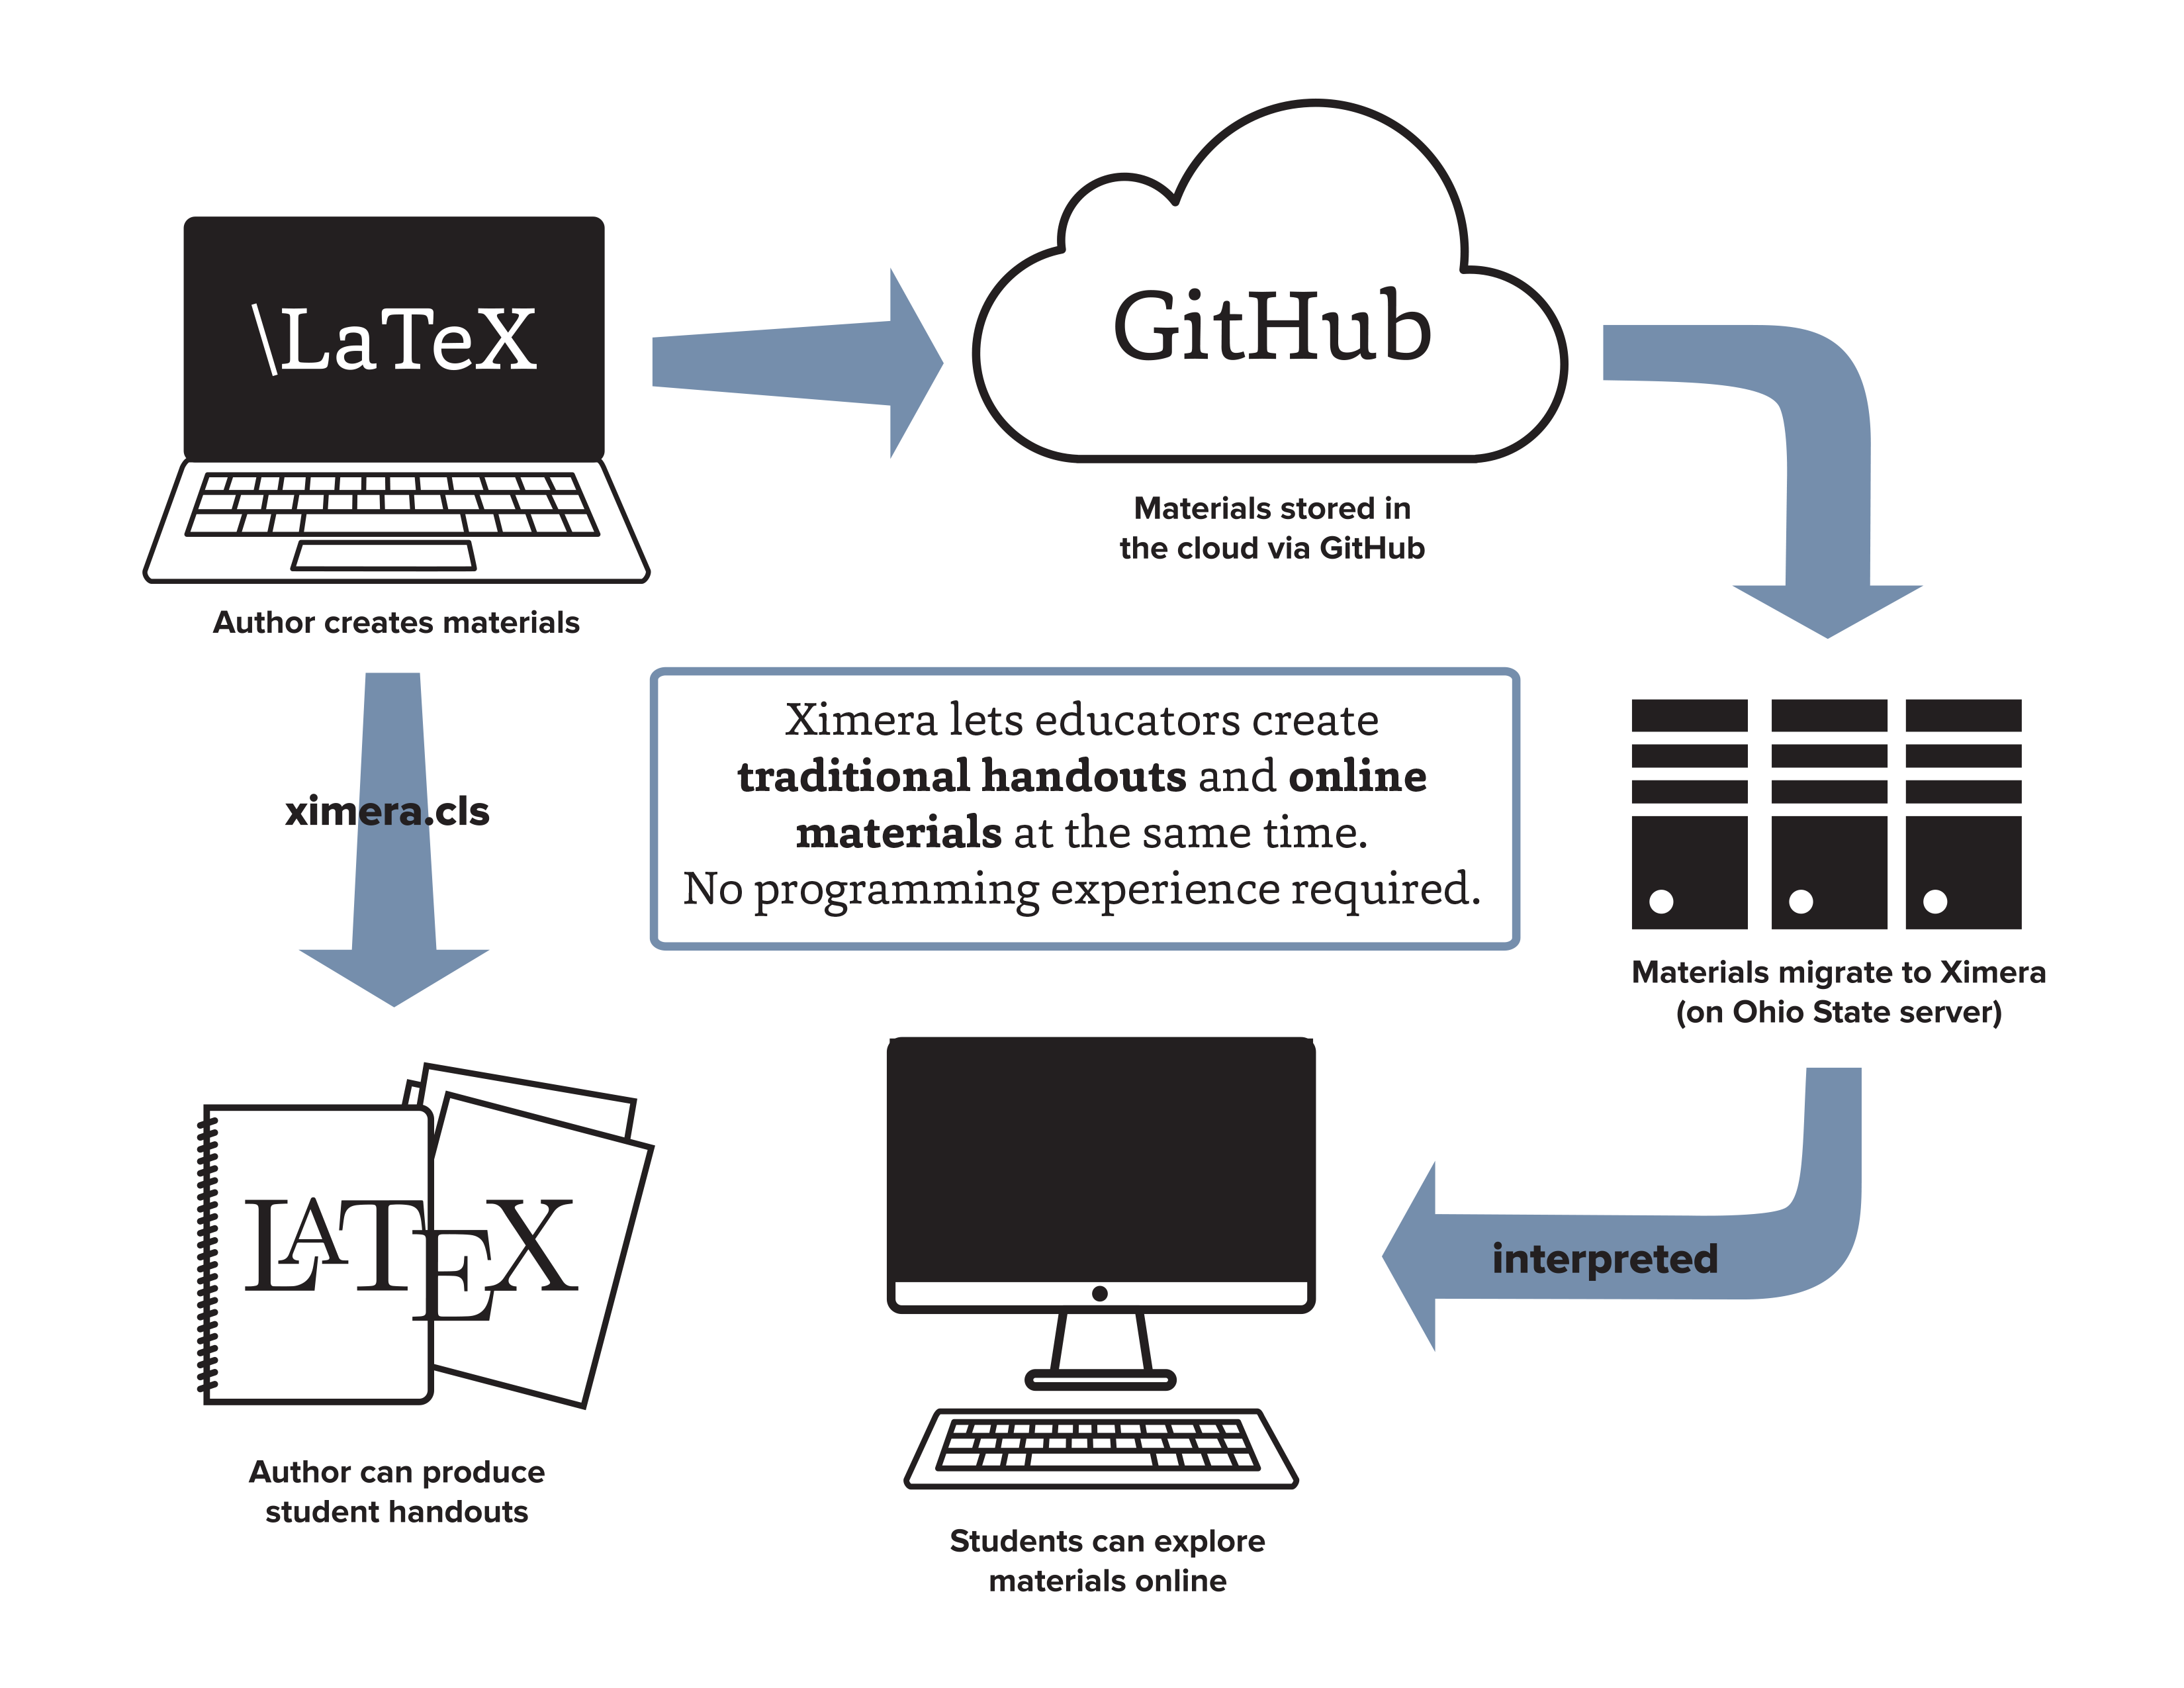
\includegraphics[scale=.25]{./XimeraGraphic.png}
\end{image}

Example courses can be found at the links below:

\begin{itemize}
\item \link[Calculus 1]{http://ximera.osu.edu/course/mooculus/calculus1}
\item \link[Calculus 2]{http://ximera.osu.edu/course/mooculus/calculus2}
\item \link[Calculus $e$]{http://ximera.osu.edu/course/mooculus/calculusE}
\item \link[Calculus 3]{http://ximera.osu.edu/course/mooculus/calculus3}
\item \link[Linear Algebra]{http://ximera.osu.edu/course/mooculus/linearAlgebra}
  
\end{itemize}


\end{document}
